\subsubsection{Tarjetas gráficas}

Una tarjeta gráfica (También conocida como tarjeta de video, placa de vídeo, o adaptador de pantalla) es una tarjeta de expansión de la computadora que contiene una unidad de procesamiento gráfico que procesa datos de salida gráfica a un dispositivo de visualización, como un monitor.

Las tarjetas gráficas son comúnmente usadas para jugar a videojuegos, usar software multimedia como software de edición de imágenes, de edición de video, de modelado 3D, o minar criptomonedas \cite{wikitarjetagrafica}.

Componentes principales \cite{juanpblogs}:

\begin{itemize}
  \item GPU
  \item VRAM
  \item RAMDAC
  \item Salidas
  \item Interfaces con la placa base
  \item Dispositivos refrigerantes
  \item Alimentación
\end{itemize}

\begin{figure}[H]
  \centering
  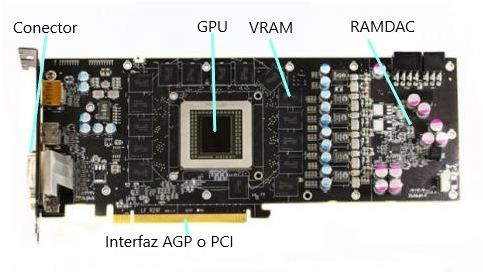
\includegraphics[scale=0.8]{imagenes/componentes-tarjeta.png}
  \caption{Componentes de la tarjeta gráfica}
\end{figure}

\begin{figure}[H]
  \centering
  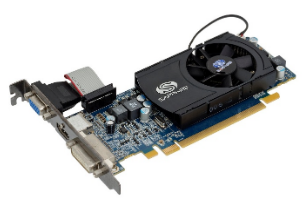
\includegraphics[scale=0.9]{imagenes/dispositivos-refrigerante.png}
  \caption{Dispositivos refrigerantes y salidas}
\end{figure}

Ejemplos:

NVIDIA GeForce RTX 4070 Ti – Muy potente, ideal para gaming y trabajo con IA.

AMD Radeon RX 6800 XT – Competencia directa de las GPUs de NVIDIA.

Intel Arc A770 – Una opción emergente de Intel.

\subsubsection{Tarjetas de sonido}

Una tarjeta de sonido o placa de sonido es una tarjeta de expansión para computadoras que permite la salida de audio controlada por un programa informático llamado controlador (driver).

El uso típico de las tarjetas de sonido consiste en hacer, mediante un programa que actúa de mezclador, que las aplicaciones multimedia del componente de audio suenen y puedan ser gestionadas. Estas aplicaciones incluyen composición de audio y en conjunción con la tarjeta gráfica también puede hacerse una edición de vídeo, presentaciones multimedia y entretenimiento (videojuegos). Algunos equipos (como computadoras personales) tienen la tarjeta ya integrada a la placa base, mientras que otros requieren tarjetas de expansión. También hay equipos que por su uso (como por ejemplo servidores) no requieren de dicha función \cite{tuhome}.

Su apariencia física no difiere demasiado de la mayoría de tarjetas de expansión que se hayan visto antes. Es decir, se trata de placas planas de plástico en cuya superficie hay una serie de microcircuitos integrados. Su forma es rectangular, y en uno de sus extremos presentan una superficie de metal perpendicular y alargada con varios conectores, mientras que en el otro la placa es plana \cite{conceptarjsond}.

\begin{figure}[H]
  \centering
  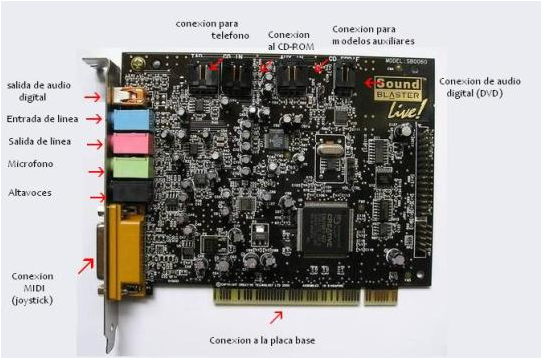
\includegraphics[scale=0.8]{imagenes/tarjeta-sonido.png}
  \caption{Partes de una tarjeta de sonido}
\end{figure}

Ejemplos:

Creative Sound Blaster Z SE – Muy buena para gamers y audiófilos.

ASUS Xonar AE – Tarjeta de sonido PCIe con buena calidad de audio.

Behringer UMC22 – Tarjeta externa para grabación de audio profesional (más común en estudios).

\subsubsection{Tarjetas de red}

La tarjeta de red, también conocida como placa de red, adaptador de red, adaptador LAN, Interfaz de red física, o sus términos en inglés network interface card o network interface controller (NIC) es un componente de hardware que conecta una computadora a una red informática y que posibilita compartir recursos (como archivos, discos duros enteros, impresoras, e internet) entre dos o más computadoras, es decir, en una red de computadoras \cite{wikitarjred}.

\textbf{Tipos de tarjeta de red}

Existen diversos tipos de tarjetas, placas o adaptadores de red, en función del tipo de cableado o arquitectura de red:

\begin{itemize}
  \item Token Ring
  \item ARCNET
  \item Ethernet
  \item Wi-Fi
\end{itemize}

\begin{figure}[H]
  \centering
  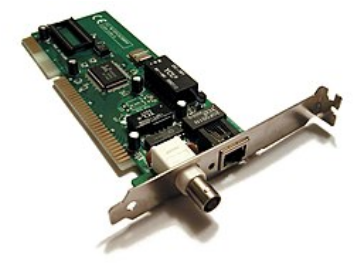
\includegraphics[scale=0.8]{imagenes/tarjeta-red.png}
  \caption{Tarjeta de red}
\end{figure}

Ejemplos:

TP-Link TG-3468 – Tarjeta Ethernet PCIe de 1 Gbps.

Intel Wi-Fi 6 AX200 – Tarjeta interna con Wi-Fi 6 y Bluetooth.

ASUS PCE-AX3000 – Tarjeta Wi-Fi de alto rendimiento.

\subsubsection{Tarjetas controladoras}

Todos los dispositivos periféricos, tanto internos como externos necesitan valerse de algún medio para comunicarse entre ellos y las computadoras. Algunas veces les llaman controladores, interfaces, puertos o adaptadores.

Básicamente un controlador es un traductor entre la CPU y el dispositivo periférico como discos duros, disquete, teclado o monitor \cite{tarjcontrol}.

\begin{figure}[H]
  \centering
  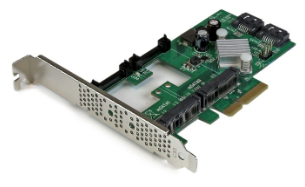
\includegraphics[scale=0.9]{imagenes/tarjeta-controladora.png}
  \caption{Tarjeta controladora RAID}
\end{figure}

Ejemplos:


Delock 89384 – Controladora PCIe para discos SSD M.2 NVMe.

LSI SAS 9211-8i – Muy usada en servidores para conectar varios discos duros SAS o SATA.

StarTech PEXSAT34RH – Agrega puertos SATA extra a tu PC.

\subsubsection{Tarjetas de expansión}

La tarjeta de expansión es un tipo de dispositivo con diversos circuitos integrados (chips) y controladores, que insertada en su correspondiente ranura de expansión sirve para expandir las capacidades de la computadora a la que se inserta. Las tarjetas de expansión más comunes sirven para añadir memoria, controladoras de unidad de disco, controladoras de vídeo, puertos serie o paralelo y dispositivo de módem interno \cite{wikitarjexpan}.

Tipos \cite{josito}:

\begin{itemize}
  \item PCI
  \item PCI Express
  \item AGP
\end{itemize}

\begin{figure}[H]
  \centering
  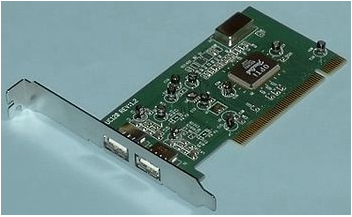
\includegraphics[scale=0.9]{imagenes/tarjeta-expansion.png}
  \caption{Tarjeta de expansión con dos puertos USB 1.1 para ranura PCI}
\end{figure}

Ejemplos:

Inateck PCIe USB 3.0 Card – Agrega puertos USB 3.0.

IOCREST PCIe to Serial Card – Añade puertos seriales RS232.

TP-Link UB500 – Adaptador USB Bluetooth 5.0 (tarjeta externa pequeña).
